\documentclass[font=default]{mpltx}
\usepackage{bm, ctex, array}
\usepackage{subfigure}
\usepackage{multirow}
% 以下至 \begin{document} 都仅是本文件为了方便额外定义的命令, 写报告时不需要.
\hypersetup{colorlinks=false}% 超链接带颜色
\usepackage{xcolor}
% 以上是本文件为了方便额外定义的命令, 写报告时不需要.
\linespread{1.5}
\begin{document}

\title{穆斯堡尔效应} % 切合报告内容, 简短明确, 可以不同于讲义
\author{MaskedName} % 这里 \emailphone 一定要紧跟在 \author 后方
\emailphone{MyMail@stu.pku.edu.cn}{Tel}
% 如果改用 \email 则仅需要邮箱参数
\affiliation{北京大学物理学院\quad 学号: StudentID}
\date{\zhdate{2024/10/31}}
\begin{abstract}
固体中的原子核在发射或者吸收$\gamma$射线的时候有一定的概率不会发生核反冲,这就是穆斯堡尔效应。通过基于Geant4开发的mossbSim软件,我们能对穆斯堡尔效应进行模拟。在本实验中,我们模拟了探测器厚度、源与样品距离等参数对穆斯堡尔谱的影响,并通过对穆斯堡尔谱的分析,测量了$^{57}$Fe核能级的塞曼分裂、同质异能移位和电四极分裂等超精细结构。此外,我们还使用专业软件模拟了1居里$_{27}^{57}$Co核素对人体的辐射大小。
\end{abstract}
\keywords{穆斯堡尔效应,穆斯堡尔谱,超精细结构,蒙特卡罗模拟}

\maketitle

\section{引言}
因为$\gamma$射线的能量较高,所以我们会观察到当$\gamma$射线和自由原子核相互作用的时候,会有显著的反冲,而这又会使得$\gamma$射线能量相对于核能级差出现移动。但是在1957年,还是博士生的穆斯堡尔在实验室中发现,固体中的$^{191}$Ir核在发射或者吸收$\gamma$射线的时候有一定的概率不会发生核反冲,即穆斯堡尔效应。该工作在1958年发表,在短短的三年后,即1961年,穆斯堡尔就获得了诺贝尔物理学奖。

穆斯堡尔谱拥有非常窄的线宽和非常高的分辨率,在测量核能级的超精细结构、确定核磁矩、评估核激发态的寿命、以及探测固体内部的电场和磁场强度方面发挥着重要作用。此外,穆斯堡尔谱还广泛应用于固体晶格振动的研究。这一技术已成为化学、磁学、固体物理学、生物学和冶金学等多个学科领域内不可或缺的研究工具。

穆斯堡尔效应的发现引领了一系列重要实验,其中包括著名的Pound-Rebka实验。该实验在1959年利用位于哈佛Jefferson实验室楼顶和地面的$\gamma$射线发射和吸收体,精确测量了光子的引力红移现象,证实了相对论的预言\cite{pound-rebka}。通过穆斯堡尔谱,科学家们能够深入探究原子核的超精细结构。在本实验中,我们采用了多普勒效应来微调入射的无反冲$\gamma$光子的能量,从而精确分辨不同原子核能级的超精细结构。通过这种方法,我们能够研究在不同实验条件下穆斯堡尔谱的差异。

\section{理论}
\subsection{穆斯堡尔效应原理}
一般来说,对于$\gamma$射线的吸收和发射过程,其谱线是洛伦兹线型,谱线强度$I$和光子能量$E$之间的关系为$$I(E)\propto\frac{1}{(E-E_0)^2+\frac{\hbar^2}{4\tau^2}}.$$在自由电子核发出$\gamma$光子的过程中,由于核的反冲,发出光子的能量会发生变化,由动量守恒得到核的反冲能为$$E_R=\frac{P_\gamma^2}{2m_N}\approx\frac{E_0^2}{2m_Nc^2},$$其中$P_\gamma$、$E_0^2$为出射光子的动量和能量,$m_N$为核的质量。而由能量守恒,入射/出射光子的$E_0$会变为$E_0\pm E_R$。对于$^{57}$Fe的$E_0=14.4$ keV激发态而言,$\tau\approx0.14\ {\rm \mu s}$,对应$\Gamma\approx4.9\times10^{-9}$ eV的尖锐谱线。而反冲给出的谱线移动$E_R\approx2\times10^{-3}\ {\rm eV}\gg\Gamma$,因此$E_0\pm E_R$两条发射和吸收谱线会发生分离,导致无法形成共振吸收。

室温下,热运动引起的多普勒效应导致谱线展宽,从而使发射和吸收谱线发生重叠,进而发生共振吸收。但是由于多普勒展宽的效果,即使忽略核反冲,有效吸收截面也要减小一个因子$\Gamma/D_T\approx2.5\times10^{-7}$。因此仅仅依靠热运动的多普勒展宽是难以观察到共振吸收的。

但是,穆斯堡尔发现:当发射或者接受$\gamma$射线的核被嵌在固体中时,出现无反冲$\gamma$射线发射或者共振吸收的概率是相当大的。而对无反冲发射常见的解释是,当核被嵌在固体中时,固体与核成为一个整体,上式的$m_N$应该用整个固体的质量代替,反冲能与自然线宽相比微不足道,完全可以认为就是0。但是这样的说法是没有办法解释为什么不是每一次发射$\gamma$光子都是无反冲的这一实验现象。实际上穆斯堡尔效应为一个量子效应,我们必须用量子力学的方法来描述这一过程。

记发射$\gamma$光子前后,包括我们所考察的衰变核A在内的所有固体的状态为$\Psi_i$和$\Psi_f$。由于发射$\gamma$光子这一过程中,我们可以认为$\gamma$光子与原子核A的作用是瞬时的,而瞬时的相互作用能够造成有限的影响,说明瞬时的相互作用趋于无穷大。因此我们可以忽略与发射$\gamma$光子无关的,固体内部其他粒子相互作用的哈密顿量,或者说,我们将核A看作自由的原子核。这样,发射一个$\gamma$光子对固体的影响仅仅限于:发射光子的那个核得到了一个动量$P_\gamma$,即$$\Psi_f=e^{i\bm{k}_\gamma\cdot \bm{R}_A}\Psi_i,$$其中$\bm{R}_A$是原子核A的位置,$\bm{k}_\gamma$是出射$\gamma$光子的波矢。这样我们就可以计算发射一个$\gamma$光子后固体系统的平均能量变化为
$$\begin{aligned}
  \langle\Delta E\rangle&=\langle\Psi_f|\hat{H}_0|\Psi_f\rangle-\langle\Psi_i|\hat{H}_0|\Psi_i\rangle\\
  &=\langle\Psi_i|e^{-i\bm{k}_\gamma\cdot \bm{R}_A}\hat{H}_0e^{i\bm{k}_\gamma\cdot \bm{R}_A}|\Psi_f\rangle-\langle\Psi_i|\hat{H}_0|\Psi_i\rangle.
\end{aligned}$$其中$\hat{H}_0$是与$\gamma$光子发射无关,即固体本身的哈密顿量。若晶体相对于观察者静止,可以计算得到$$\langle\Delta E\rangle=\frac{\hbar^2k_\gamma^2}{2m_A}=E_R.$$这表明,即使核被嵌在晶体中,发射一个$\gamma$光子传递的反冲能和核是自由时完全一样。

然而,测定固体的吸收、发射谱,本质上正是对固体能量的观测;这一观测导致固体波函数坍缩至某一能量本征态,其中有一定概率回到初态,此即对应无反冲情形。无反冲分数$f$可由终态与初态的交叠加以刻画:$$f=|\langle \Psi_f|\Psi_i\rangle|^2.$$这就是穆斯堡尔效应的基本图像。
\subsection{超精细相互作用}
\begin{figure}
  \centering
  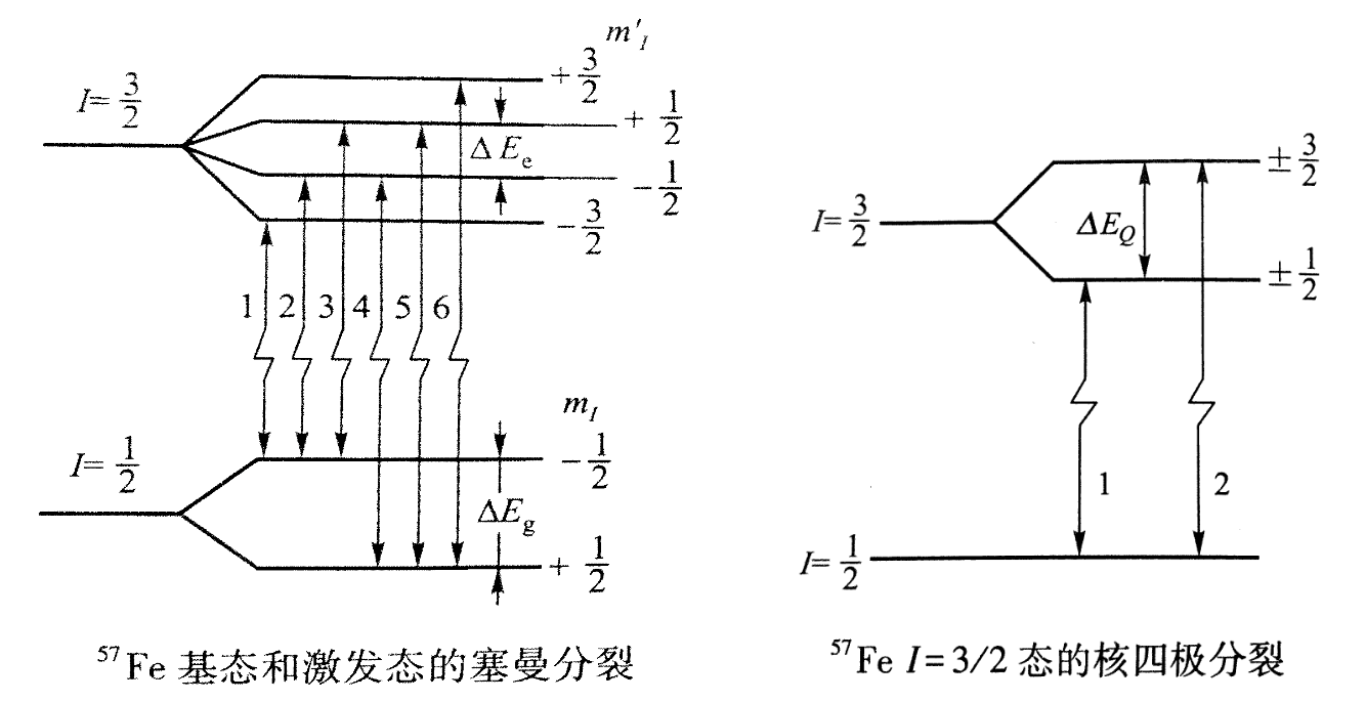
\includegraphics[width=0.6\textwidth]{fig/fine_struct.png}
  \caption{$^{57}$Fe超精细相互作用导致的能级分裂示意图}
  \label{fig:hfs}
\end{figure}
因为穆斯堡尔谱十分尖锐,而且从源发出的$\gamma$射线相对于吸收体的能量移动能够到达十分高的精度,因此其特别适合研究超精细相互作用,超精细相互作用主要有如下三种:

1. \textbf{核塞曼分裂}:原子核的磁偶极矩$\mu$和原子核处的磁场$B$会发生磁偶极相互作用,从而导致塞曼分裂,相邻能级之间的间距为$$\Delta E= g_N\mu_NB.$$其中$g_N$为原子核的郎德因子,$\mu_N=e\hbar/2m_p$($m_p$是质子质量)是核磁子。对于$^{57}$Fe而言,如\autoref{fig:hfs} 所示,塞曼效应会导致六条相近的谱线。

2. \textbf{电四极矩分裂}:由于核电荷的分布不是球形对称的,在电场梯度的作用下,核能级会移动并且分裂成不同能级,这就是电四极矩分裂。四极分裂后,激发态两个能级之间的能级差为$$\Delta E = \frac{e^2Q\cdot q}{2}.$$其中$eq$对应电场梯度主分量,$eQ$对应电四极矩主分量。对于$^{57}$Fe而言,如\autoref{fig:hfs} 所示,电四极矩分裂会导致两条谱线。

3. \textbf{同质异能移位}:由于原子核具有一定的体积,核外的s电子在核内会有一定的概率分布,又因为核在激发的时候半径会发生变化,所以会导致能量发生变化,这就是同质异能移位。放射源核吸收体通常都会有大小不同的同质异能移位,因此实际讨论以及测量的同质异能移位为不同原子核之间的差值。
\section{实验内容}
\subsection{实验装置}
考虑到放射性源的限制,本次实验通过计算机模拟的方式进行。我们使用了基于Geant4软件包开发的mossbSim软件,专门用于模拟穆斯堡尔效应。通过该软件,我们对探测器的不同厚度、源与样品之间的不同距离,以及$\alpha$-Fe和硝普酸钠等不同样品进行了模拟计算。在模拟过程中,我们让穆斯堡尔源以10 Hz的频率进行往返匀加速运动,模拟电磁驱动的效果,并通过多普勒效应实现$\gamma$射线能量的周期性和线性调制。\autoref{fig:setup} 是穆斯堡尔效应实验的装置示意图。
\begin{figure}
  \centering
  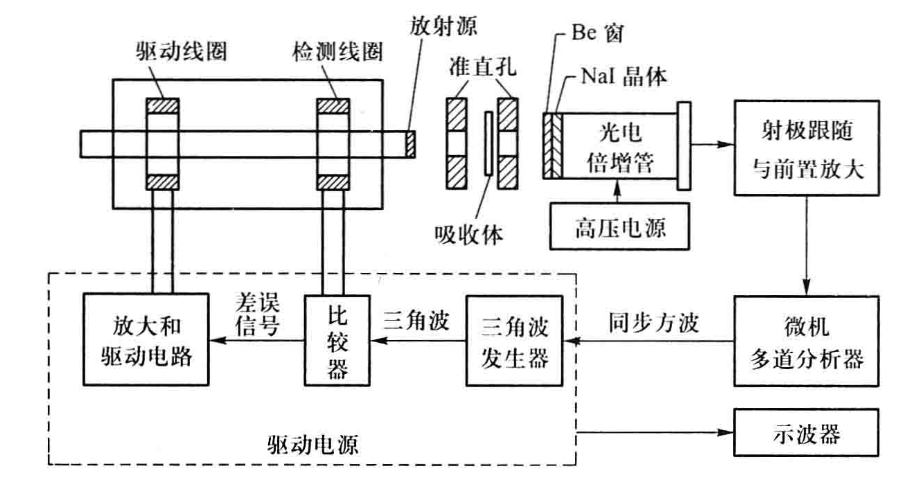
\includegraphics[width=0.6\textwidth]{fig/setup.png}
  \caption{穆斯堡尔效应实验装置示意图}
  \label{fig:setup}
\end{figure}
\subsection{实验过程}
首先进行穆斯堡尔效应实验,按照实验台或者计算机的桌面上《mossbSim操作演示》的文件说明,实现探测器厚度分别为0.13 mm和13 mm、源与样品的距离分别为5 mm和100 mm的$\alpha$-Fe样品的Geant4模拟。样品换为硝普酸钠,厚度/距离=0.13 mm/100 mm,重复实验。最后通过测量得到的谱计算道增益$K$,零速度对应的道址,$^{57}$Fe基态和第一激发态的郎德$g$因子和核磁矩大小,硝普酸钠的同质异能移位和四级裂距。

随后进行剂量实验。根据电脑Dose目录下“点源吸收剂量计算v0”说明,利用专业模型,即目录ICRP145\_HumanPhantomsAir下的bin的可执行程序,模拟1居里$_{27}^{57}$Co核素放在人体右侧1 m处的吸收剂量。
\section{实验结果与分析}
\subsection{穆斯堡尔效应实验}
首先取探测器NaI样品的厚度为0.13 mm,源与样品的距离为100 mm,得到的$^{57}$Co放射源能谱如 所示。其中X为道地址数,Y为光子计数。红色竖线为所设置的14.4 keV的$\gamma$射线产生的信号峰左、右两侧的阈值。从左往右四个能峰分别对应6.4 keV的Fe的X射线、14.4 keV的$\gamma$射线、123keV和137keV的$\gamma$射线在NaI中I元素产生的X射线逃逸后剩余能量产生的信号峰、123keV和137keV的$\gamma$射线全能峰\cite{mossbSim}。
\begin{figure}[h]
  \centering
  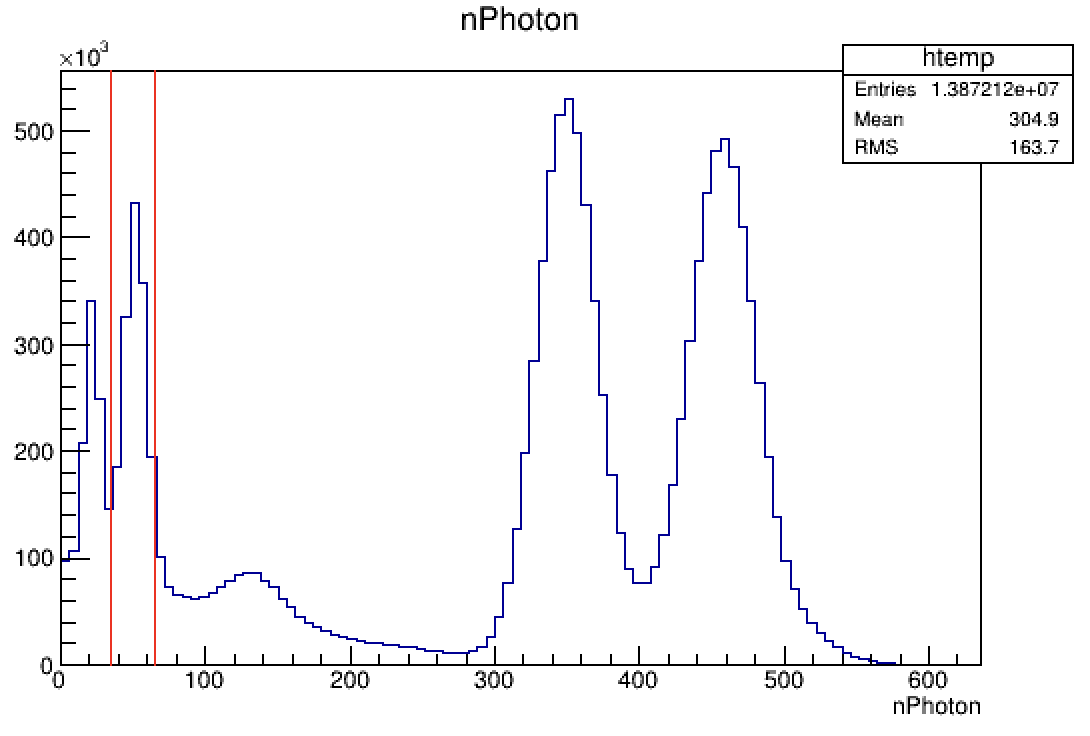
\includegraphics[width=0.6\textwidth]{fig/DetThick/0.13mm/htemp.png}
  \caption{NaI探测器厚度为0.13 mm、源与样品距离为100 mm下测量得到的$^{57}$Co能谱}
  \label{fig:htemp_0.13mm_100mm}
\end{figure}

根据\autoref{fig:htemp_0.13mm_100mm} 所示的14.4 keV峰的上下阈(红色线),可以在这个上、下阈之间观察信号对应的补偿速度的分布,也就是穆斯堡尔谱。\autoref{fig:h2_0.13mm_100mm} 是我们在探测器厚度为0.13 mm、源与样品距离为100 mm下测量得到的$\alpha$-Fe样品穆斯堡尔谱。在模拟程序中,X轴(道地址)与补偿速度$v$之间存在一个预定义的转换关系。具体来说,mossbSim软件中已经设定好,第1道对应$+v$,第256道对应$-v$,而第512道再次对应$+v$。因此,如果设定的速度变化范围覆盖了六个共振位置,那么在每个模拟周期中,将会经历两次共振,相应地,模拟得到的$\alpha$-Fe的穆斯堡尔谱图将展现出12个共振位置,并且这些位置关于第256道对称分布。
\subsubsection{计算道增益$K$}
通过Origin的``Multiple Peak Fit''功能,我们可以从\autoref{fig:h2_0.13mm_100mm} 中找到六个共振位置的道址,如\autoref{tab:h2_0.13mm_100mm} 所示。注意到右侧峰道地址随序号递增,而左侧锋随序号递减,这是因为它们分别对应着一个速度周期中的上升和下降区间。我们已知$\alpha$-Fe的$v_6-v_1=10.656$ mm/s,于是道增益$K$为
$$K=\frac{10.656}{|v_6-v_1|_{\alpha-\text{Fe}}}\ \text{mm/s}\approx6.25\times10^{-2}\ {\rm mm/s}.$$
其中$|v_6-v_1|_{\alpha-\text{Fe}}$为左右道址的结果平均得到,下面计算也类似。
\begin{figure}[h]
  \centering
  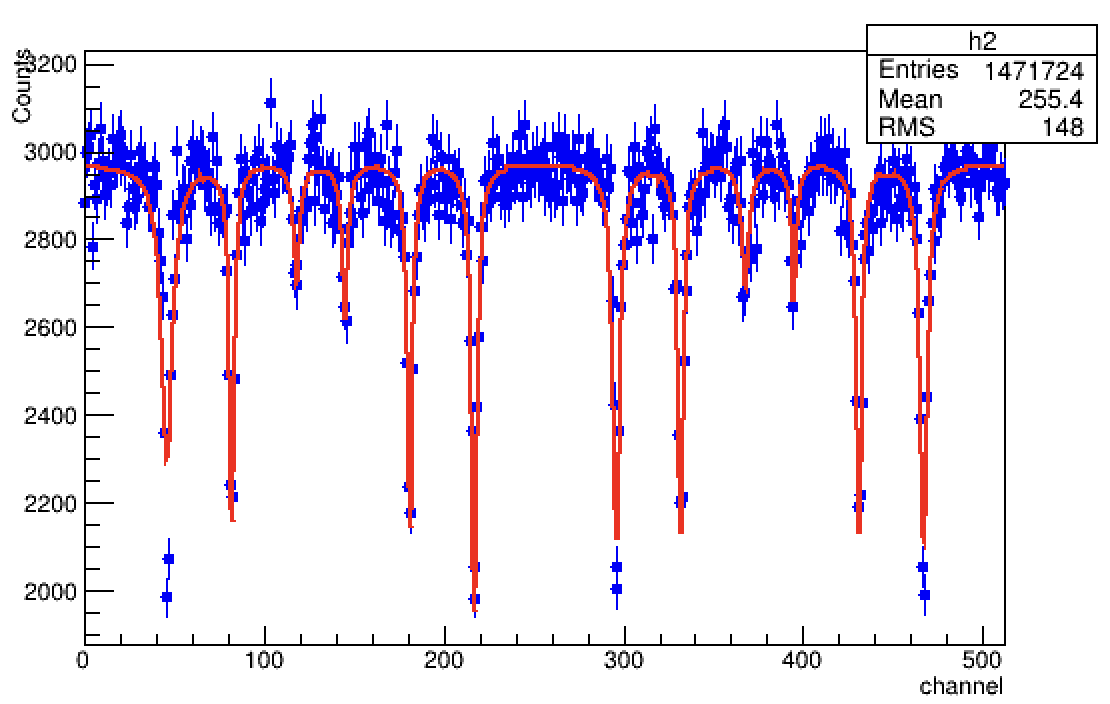
\includegraphics[width=0.6\textwidth]{fig/DetThick/0.13mm/h2.png}
  \caption{NaI探测器厚度为0.13 mm、源与样品距离为100 mm下测量得到的$\alpha$-Fe样品穆斯堡尔谱}
  \label{fig:h2_0.13mm_100mm} 
\end{figure}
\begin{table}[h]
  \centering
  \caption{$\alpha$-Fe样品穆斯堡尔谱的峰值道地址(由\autoref{fig:h2_0.13mm_100mm} 拟合得到)}
  \vspace{0.2cm}
  \label{tab:h2_0.13mm_100mm}
  \begin{tabular}{c|cccccc}
    \hline
    序号 & 1 & 2 & 3 & 4 & 5 & 6 \\\hline
		右侧峰道地址$v_R$ &	297 & 332 & 368 & 395 & 431 & 467 \\
		左侧峰道地址$v_L$ &	217 & 182 & 145 & 118 & 82 & 46 \\
    \hline
  \end{tabular}
\end{table}
\subsubsection{零速度对应的道址}
接下来我们计算零速度对应的道址。对于我们所用的源,$\alpha$-Fe六线谱的重心应该在$-0.185$ mm/s的位置(它相当于$\alpha$-Fe与Pd衬底的$^{57}$Co源之间的同质异能移位),可根据下面的公式定出$\alpha$-Fe谱的重心位置
$$v_{c,\alpha-\text{Fe}}=\frac{v_1+v_2+v_5+v_6}{4}=\left\{\begin{aligned}
  381.75,\ \mbox{右侧},\\
  131.75,\ \mbox{左侧}.
\end{aligned}\right.$$于是零速度对应的道址为
$$v_{0,\alpha-\text{Fe}}=v_c\pm\frac{-0.185\ \text{mm/s}}{K}=\left\{\begin{aligned}
  384.7,\ \mbox{右侧},\\
  128.8,\ \mbox{左侧}.
\end{aligned}\right.$$我们可以计算左右侧的零速度道址间隔为$384.7-128.8=255.9\approx256$,这表明我们的速度周期和道址是匹配的。反之,在确定道址和速度的匹配关系的前提下,我们也可以通过这一结果验证$-0.185$ mm/s这个数值的可靠性。

\subsubsection{$^{57}$Fe基态和第一激发态的郎德$g$因子和核磁矩大小}
已知$\alpha$-Fe的内磁场为$B_{\text{int}}=33.3$ T。对14.4 keV的谱线,$E_0/c=4.80766\times10^{-8}\ {\rm eV\cdot s\cdot mm^{-1}}$,比较前述塞曼分裂的能谱图\autoref{fig:hfs},我们可以通过下面公式计算得到塞曼分裂的裂距:
$$\begin{aligned}
  \Delta E_g=\frac{|v_4-v_2|+|v_5-v_3|}{2}\frac{KE_0}{c}=1.900\times10^{-7}\ {\rm eV},\\
  \Delta E_e=\frac{|v_3-v_2|+|v_5-v_4|}{2}\frac{KE_0}{c}=1.089\times10^{-7}\ {\rm eV}.
\end{aligned}$$
上面的结果都是对左侧和右侧进行平均后得到的结果。由$\Delta=g\mu_NB$,以及$\mu_N=3.152451\times10^{-8}\ {\rm eV/T}$,我们可以计算得到$g$因子和核磁矩大小:
$$\begin{aligned}
  g_g=0.183,\quad \mu_g=5.76\times10^{-9}\ {\rm eV/T},\\
  g_e=0.105,\quad \mu_e=3.30\times10^{-9}\ {\rm eV/T}.
\end{aligned}$$
\subsubsection{硝普酸钠的同质异能移位和四级裂距}
将样品换做硝普酸钠,保持探测器厚度为0.13 mm,源与样品的距离为100 mm,重复上述实验,得到的穆斯堡尔谱如\autoref{fig:Na_h2} 所示。通过拟合得到的峰值道址如\autoref{tab:Na_h2} 所示。
\begin{figure}[h]
  \centering
  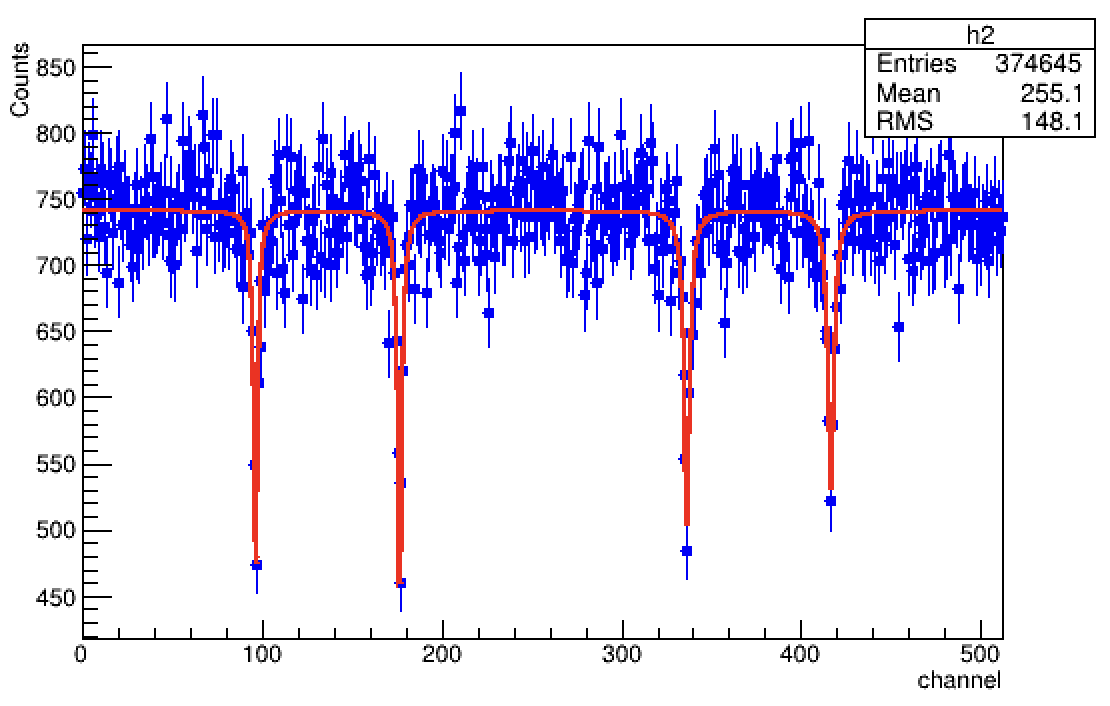
\includegraphics[width=0.6\textwidth]{fig/Na/Na_h2.png}
  \caption{NaI探测器厚度为0.13 mm、源与样品距离为100 mm下测量得到的硝普酸钠样品穆斯堡尔谱}
  \label{fig:Na_h2} 
\end{figure}
\begin{table}[h]
  \centering
  \caption{硝普酸钠样品穆斯堡尔谱的峰值道地址(由\autoref{fig:Na_h2} 拟合得到)}
  \vspace{0.2cm}
  \label{tab:Na_h2}
  \begin{tabular}{c|cc}
    \hline
    序号 & 1 & 2  \\\hline
		右侧峰道地址$v_R$ &	337 & 417  \\
		左侧峰道地址$v_L$ &	177 & 97 \\
    \hline
  \end{tabular}
\end{table}

硝普酸钠相对于$\alpha$-Fe的重心偏移量为
$$\Delta v=\left|\left(\frac{v_1+v_2}{2}\right)_{\mbox{\small{硝普酸钠}}}-v_{c,\alpha-\text{Fe}}\right|=5.00.$$于是硝普酸钠的同质异能移位为$$\Delta E=\Delta v\frac{KE_0}{c}=1.50\times10^{-8}\ {\rm eV}.$$
同样,对于硝普酸钠样品,对比上面电四极矩分裂的能谱图,我们可以计算得到电四极矩分裂的裂距:
$$\Delta E_q=|v_2-v_1|\frac{KE_0}{c}=2.40\times10^{-7}\ {\rm eV}.$$这就是$^{57}$Fe第一激发态的电四极分裂裂距。
\subsubsection{对不同参数的讨论}
对$\alpha$-Fe样品,除了0.13 mm的探测器厚度和100 mm的源与样品距离,我们还进行了探测器厚度为13 mm、源与样品距离为100 mm的实验以及探测器厚度为0.13 mm、源与样品距离为5 mm的实验。实验结果如\autoref{fig:htemp_13mm_100mm} 至\autoref{fig:h2_0.13mm_5mm} 所示。
\begin{figure}[h]
  \centering
  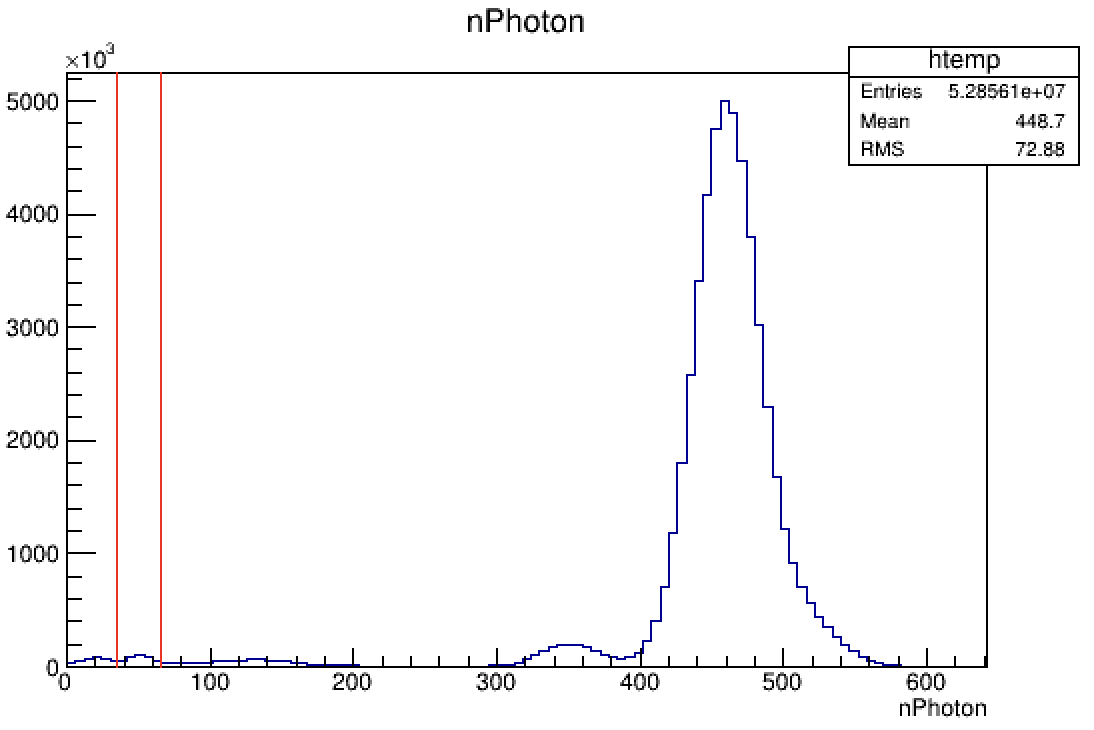
\includegraphics[width=0.6\textwidth]{fig/DetThick/13mm/htemp.png}
  \caption{探测器厚度为13 mm、源与样品距离为100 mm下测量得到的$^{57}$Co能谱}
  \label{fig:htemp_13mm_100mm}
\end{figure}
\begin{figure}[h]
  \centering
  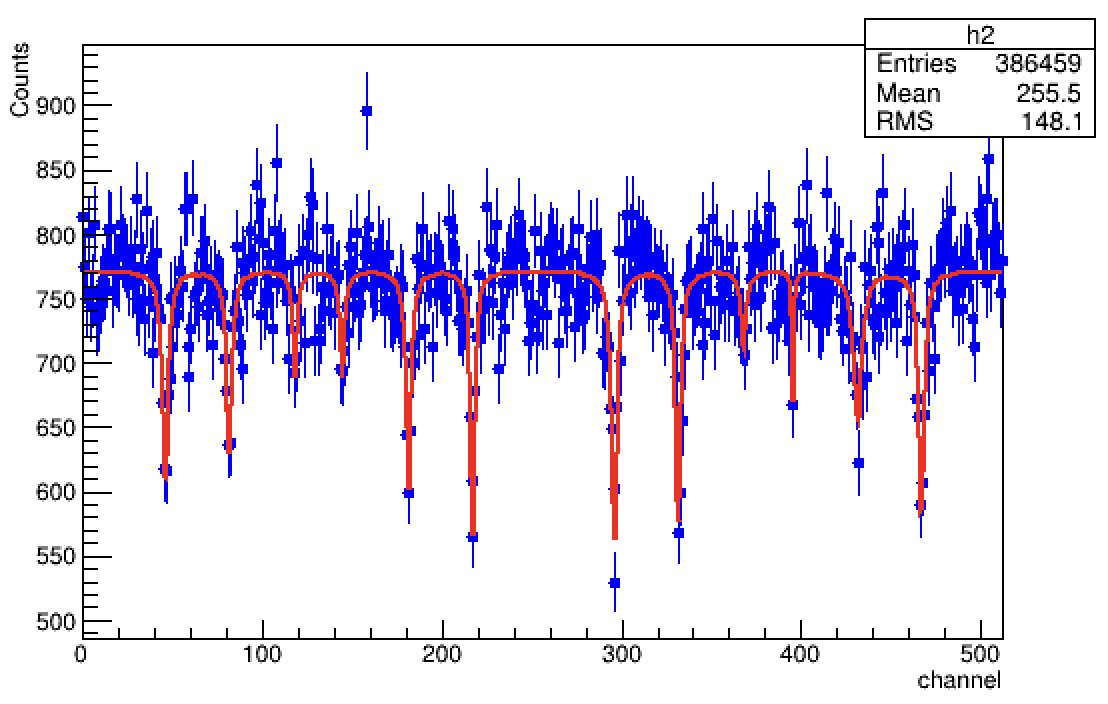
\includegraphics[width=0.6\textwidth]{fig/DetThick/13mm/h2.png}
  \caption{探测器厚度为13 mm、源与样品距离为100 mm下测量得到的$\alpha$-Fe样品穆斯堡尔谱}
  \label{fig:h2_13mm_100mm}
\end{figure}
\begin{figure}[h]
  \centering
  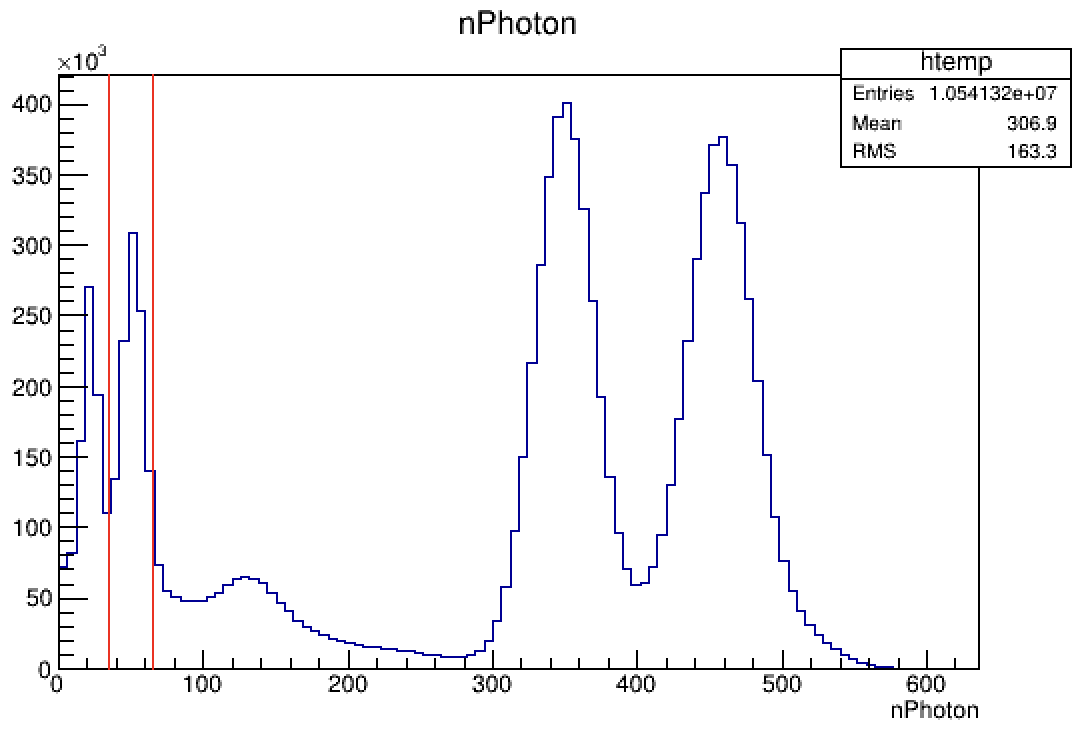
\includegraphics[width=0.6\textwidth]{fig/DistSource/5mm/htemp.png}
  \caption{探测器厚度为0.13 mm、源与样品距离为5 mm下测量得到的$^{57}$Co能谱}
  \label{fig:htemp_0.13mm_5mm}
\end{figure}
\begin{figure}[h]
  \centering
  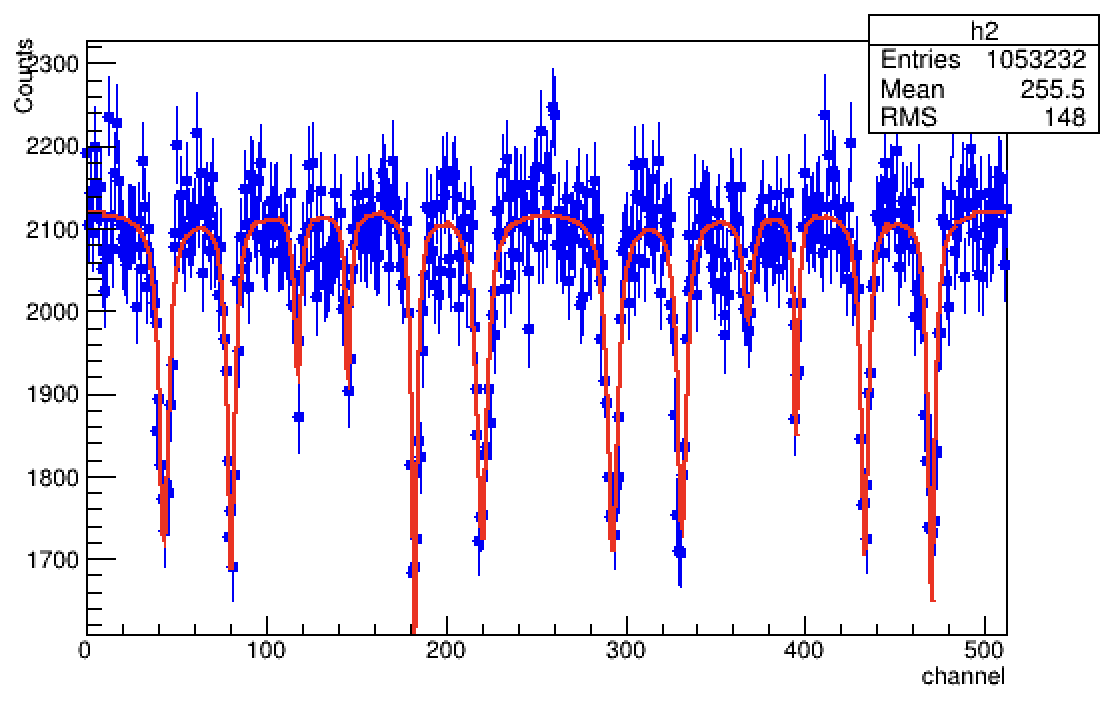
\includegraphics[width=0.6\textwidth]{fig/DistSource/5mm/h2.png}
  \caption{探测器厚度为0.13 mm、源与样品距离为5 mm下测量得到的$\alpha$-Fe样品穆斯堡尔谱}
  \label{fig:h2_0.13mm_5mm}
\end{figure}

从\autoref{fig:htemp_0.13mm_100mm} 和\autoref{fig:htemp_13mm_100mm} 可以看到,选用较薄的探测器可以压低放射源发射的123 keV和137 keV的$\gamma$射线对实验结果可能产生的影响,让更多的信号集中在14.4 keV的$\gamma$射线上。这是因为14.4 keV的$\gamma$射线实际占总的辐射比例是相对比较小的,如果用较薄的探测器进行探测,那么相对来说能量更高、穿透能力更强的123 keV和137 keV射线在探测器上的沉积能量就会比较小。反之,若选用较厚的探测器(这里我们选了13 mm作为对比),就会导致123 keV和137 keV的射线在探测器上的沉积能量比较大,从而降低14.4 keV的$\gamma$射线的信噪比。

除了探测器厚度之外,放射源与样品的距离($D$)也是影响探测结果的重要因素。对比\autoref{fig:htemp_0.13mm_5mm}、\autoref{fig:h2_0.13mm_5mm}和\autoref{fig:htemp_0.13mm_5mm}、\autoref{fig:h2_0.13mm_5mm},我们可以看到,在不同的源与样品距离下,$\gamma$射线的能谱图实际差异并不会特别大,但是源与样品的距离变近会导致穆斯堡尔谱的分辨率变差。对这一现象我们做出下面的简要分析:$D$变小时,入射到样品的$\gamma$射线入射角更大,大角度入射的比例增加。当$D=5$ mm时,入射角较小和较大的射线不能同时满足共振条件,因此穆斯堡尔谱分辨率较差。而当$D=100$ mm时,入射角度较小,样品上有更大的区域能够发生吸收共振,从而探测到的峰会更加尖锐。
\subsection{剂量实验}
通过专业模型,我们模拟了1居里$_{27}^{57}$Co核素放在人体右侧1 m处的吸收剂量。部分数据如\autoref{fig:doseRes} 所示。我们通过下面公式可以计算一秒人体吸收的辐射剂量(单位:Gy,1 Gy=1 J/kg):
$$D=3.7\times10^{10}\times\frac{1}{M}\sum_{i=\text{Organ ID}}\text{Organ Mass}_i\times\text{Dose}_i=8.9\times10^{-8}\ {\rm Gy}.$$其中$M$是人体质量,$M=\sum_{i}\text{Organ Mass}$。
\begin{figure}[h]
  \centering
  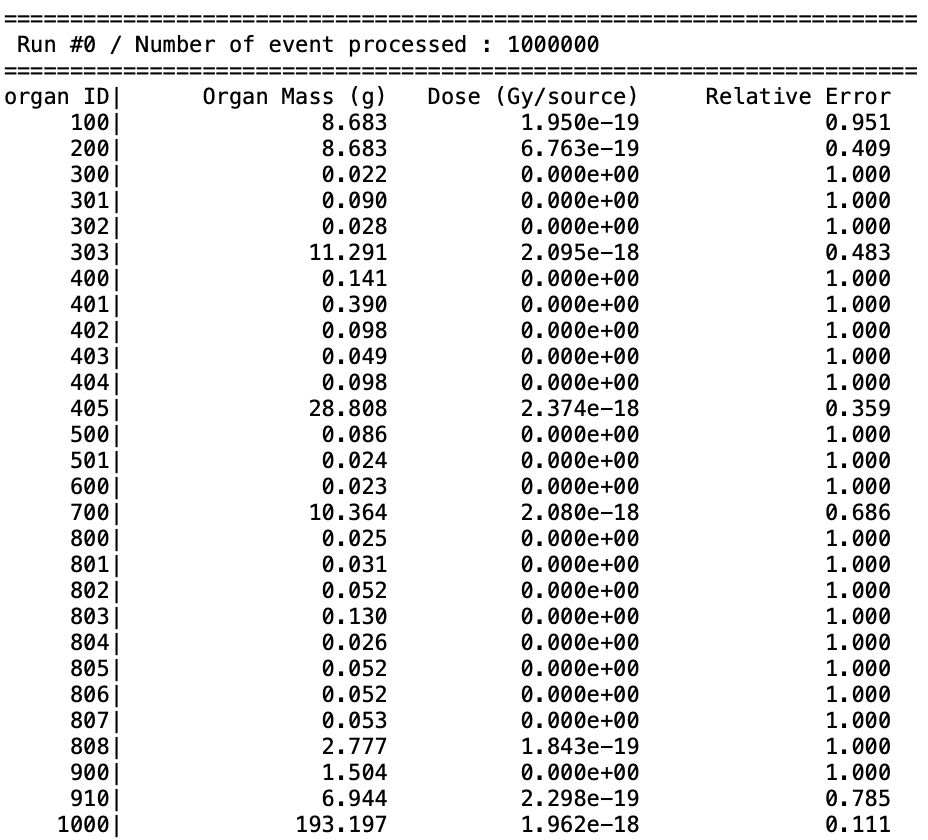
\includegraphics[width=0.4\textwidth]{fig/doseRes.png}
  \caption{$_{27}^{57}$Co核素放在人体右侧1 m处人体受到的辐射剂量,organ ID是身体不同部位器官的编号}
  \label{fig:doseRes}
\end{figure}

计算完辐射剂量后,我们用下面公式计算剂量当量:$H=DQN$(单位:Sv,1 Sv=1 J/kg),其中$D$为吸收剂量,$Q$为品质因数(x,$\gamma$,$\beta$的$Q$通常为1;中子,质子,离子、$\alpha$射线为25),$N=1$(辐照条件的改变的修正)。于是我们得到人体在一小时的辐射剂量当量为$3.2\times10^{-4}$ Sv。如果允许年剂量当量$H$是20 mSv,可知人一年内最多在这样的环境中工作62小时。

\section{结论}
本实验通过mossbSim软件对穆斯堡尔效应进行模拟,以$^{57}$Co作为$\gamma$射线源,利用多普勒效应微调制光子能量,获得了$\alpha$-Fe和硝酸普纳样品的穆斯堡尔谱。在此基础上,我们通过分析穆斯堡尔谱计算了道增益$K$和零速度对应的道址,并利用已经校准的谱研究$^{57}$Fe核的超精细结构。通过模拟计算,我们得到了$\alpha$-Fe的同质异能移位和四级裂距,分别为$1.50\times10^{-8}\ {\rm eV}$和$2.403\times10^{-7}\ {\rm eV}$。我们还计算了$^{57}$Fe基态和第一激发态的郎德$g$因子和核磁矩大小,分别为$g_g=0.183$、$\mu_g=5.76\times10^{-9}\ {\rm eV/T}$和$g_e=0.105$、$\mu_e=3.30\times10^{-9}\ {\rm eV/T}$。

最后,我们讨论了探测器厚度和源与样品距离对实验结果的影响,以及通过专业模型模拟了$^{57}$Co对人体的辐射剂量。计算表明人一年内最多在一居里$^{57}$Co辐射的环境中工作62小时。
\section{致谢}
感谢王思广老师在实验中的细致指导和耐心帮助。
\begin{thebibliography}{}
  \bibitem{pound-rebka} Pound R.V. Rebka Jr G.A. Gravitational red-shift in nuclear resonance[J]. Physical Review Letters, 1959, 3(9): 439.
  \bibitem{book} 吴思诚, 荀坤. 近代物理实验(第四版)[M]. 北京: 高等教育出版社, 2015.
  \bibitem{mossbSim} 王思广, 罗棱尹, 贾春燕. 使用mossbSim软件模拟穆斯堡尔实验[J]. 物理实验, 2021, 41(01):15-21. DOI:10.19655/j.cnki.1005-4642.2021.01.003.
\end{thebibliography}

\appendix

\section{思考题}
\subsection{在发射(吸收)$\gamma$射线后,核的质量实际上会有所下降(上升),这会带来什么后果,为什么仍然能够观察到$\gamma$射线的共振吸收呢?}
核质量的改变会导致穆斯堡尔峰的移动。而由于我们用多普勒效应进行调制$\gamma$光子能量的范围足够大,因此我们仍然可以在这个范围内看到穆斯堡尔峰的共振吸收。

\subsection{请解释为什么源或吸收体较厚的时候会导致谱的展宽?}
实验报告中对此现象做过粗略的解释,\autoref{fig:htemp_13mm_100mm} 中的较宽谱主要是因为123 keV和137 keV射线在探测器上的沉积能量比较大。同时如果源的厚度较大的话,从中放出的$\gamma$射线可能会受到一定的散射,这也会导致谱的展宽。

\subsection{在计算$\alpha$-Fe的重心位置时为何没有用到$v_3$和$v_4$?}
这是因为$v_3$和$v_4$处的共振峰相对比较小,展宽相对于其他峰更大,如果用这两个峰进行计算,可能会导致比较大的误差。


\end{document}
